\documentclass[1p]{elsarticle_modified}
%\bibliographystyle{elsarticle-num}

%\usepackage[colorlinks]{hyperref}
%\usepackage{abbrmath_seonhwa} %\Abb, \Ascr, \Acal ,\Abf, \Afrak
\usepackage{amsfonts}
\usepackage{amssymb}
\usepackage{amsmath}
\usepackage{amsthm}
\usepackage{scalefnt}
\usepackage{amsbsy}
\usepackage{kotex}
\usepackage{caption}
\usepackage{subfig}
\usepackage{color}
\usepackage{graphicx}
\usepackage{xcolor} %% white, black, red, green, blue, cyan, magenta, yellow
\usepackage{float}
\usepackage{setspace}
\usepackage{hyperref}

\usepackage{tikz}
\usetikzlibrary{arrows}

\usepackage{multirow}
\usepackage{array} % fixed length table
\usepackage{hhline}

%%%%%%%%%%%%%%%%%%%%%
\makeatletter
\renewcommand*\env@matrix[1][\arraystretch]{%
	\edef\arraystretch{#1}%
	\hskip -\arraycolsep
	\let\@ifnextchar\new@ifnextchar
	\array{*\c@MaxMatrixCols c}}
\makeatother %https://tex.stackexchange.com/questions/14071/how-can-i-increase-the-line-spacing-in-a-matrix
%%%%%%%%%%%%%%%

\usepackage[normalem]{ulem}

\newcommand{\msout}[1]{\ifmmode\text{\sout{\ensuremath{#1}}}\else\sout{#1}\fi}
%SOURCE: \msout is \stkout macro in https://tex.stackexchange.com/questions/20609/strikeout-in-math-mode

\newcommand{\cancel}[1]{
	\ifmmode
	{\color{red}\msout{#1}}
	\else
	{\color{red}\sout{#1}}
	\fi
}

\newcommand{\add}[1]{
	{\color{blue}\uwave{#1}}
}

\newcommand{\replace}[2]{
	\ifmmode
	{\color{red}\msout{#1}}{\color{blue}\uwave{#2}}
	\else
	{\color{red}\sout{#1}}{\color{blue}\uwave{#2}}
	\fi
}

\newcommand{\Sol}{\mathcal{S}} %segment
\newcommand{\D}{D} %diagram
\newcommand{\A}{\mathcal{A}} %arc


%%%%%%%%%%%%%%%%%%%%%%%%%%%%%5 test

\def\sl{\operatorname{\textup{SL}}(2,\Cbb)}
\def\psl{\operatorname{\textup{PSL}}(2,\Cbb)}
\def\quan{\mkern 1mu \triangleright \mkern 1mu}

\theoremstyle{definition}
\newtheorem{thm}{Theorem}[section]
\newtheorem{prop}[thm]{Proposition}
\newtheorem{lem}[thm]{Lemma}
\newtheorem{ques}[thm]{Question}
\newtheorem{cor}[thm]{Corollary}
\newtheorem{defn}[thm]{Definition}
\newtheorem{exam}[thm]{Example}
\newtheorem{rmk}[thm]{Remark}
\newtheorem{alg}[thm]{Algorithm}

\newcommand{\I}{\sqrt{-1}}
\begin{document}

%\begin{frontmatter}
%
%\title{Boundary parabolic representations of knots up to 8 crossings}
%
%%% Group authors per affiliation:
%\author{Yunhi Cho} 
%\address{Department of Mathematics, University of Seoul, Seoul, Korea}
%\ead{yhcho@uos.ac.kr}
%
%
%\author{Seonhwa Kim} %\fnref{s_kim}}
%\address{Center for Geometry and Physics, Institute for Basic Science, Pohang, 37673, Korea}
%\ead{ryeona17@ibs.re.kr}
%
%\author{Hyuk Kim}
%\address{Department of Mathematical Sciences, Seoul National University, Seoul 08826, Korea}
%\ead{hyukkim@snu.ac.kr}
%
%\author{Seokbeom Yoon}
%\address{Department of Mathematical Sciences, Seoul National University, Seoul, 08826,  Korea}
%\ead{sbyoon15@snu.ac.kr}
%
%\begin{abstract}
%We find all boundary parabolic representation of knots up to 8 crossings.
%
%\end{abstract}
%\begin{keyword}
%    \MSC[2010] 57M25 
%\end{keyword}
%
%\end{frontmatter}

%\linenumbers
%\tableofcontents
%
\newcommand\colored[1]{\textcolor{white}{\rule[-0.35ex]{0.8em}{1.4ex}}\kern-0.8em\color{red} #1}%
%\newcommand\colored[1]{\textcolor{white}{ #1}\kern-2.17ex	\textcolor{white}{ #1}\kern-1.81ex	\textcolor{white}{ #1}\kern-2.15ex\color{red}#1	}

{\Large $\underline{12n_{0498}~(K12n_{0498})}$}

\setlength{\tabcolsep}{10pt}
\renewcommand{\arraystretch}{1.6}
\vspace{1cm}\begin{tabular}{m{100pt}>{\centering\arraybackslash}m{274pt}}
\multirow{5}{120pt}{
	\centering
	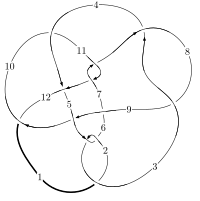
\includegraphics[width=112pt]{../../../GIT/diagram.site/Diagrams/png/2587_12n_0498.png}\\
\ \ \ A knot diagram\footnotemark}&
\allowdisplaybreaks
\textbf{Linearized knot diagam} \\
\cline{2-2}
 &
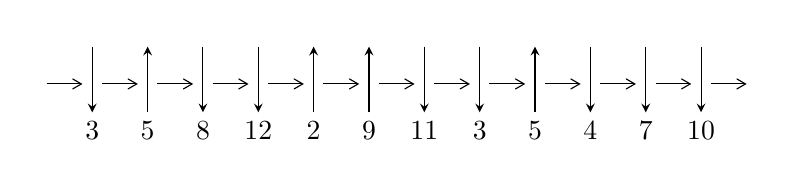
\begin{tikzpicture}[x=20pt, y=17pt]
	% nodes
	\node (C0) at (0, 0) {};
	\node (C1) at (1, 0) {};
	\node (C1U) at (1, +1) {};
	\node (C1D) at (1, -1) {3};

	\node (C2) at (2, 0) {};
	\node (C2U) at (2, +1) {};
	\node (C2D) at (2, -1) {5};

	\node (C3) at (3, 0) {};
	\node (C3U) at (3, +1) {};
	\node (C3D) at (3, -1) {8};

	\node (C4) at (4, 0) {};
	\node (C4U) at (4, +1) {};
	\node (C4D) at (4, -1) {12};

	\node (C5) at (5, 0) {};
	\node (C5U) at (5, +1) {};
	\node (C5D) at (5, -1) {2};

	\node (C6) at (6, 0) {};
	\node (C6U) at (6, +1) {};
	\node (C6D) at (6, -1) {9};

	\node (C7) at (7, 0) {};
	\node (C7U) at (7, +1) {};
	\node (C7D) at (7, -1) {11};

	\node (C8) at (8, 0) {};
	\node (C8U) at (8, +1) {};
	\node (C8D) at (8, -1) {3};

	\node (C9) at (9, 0) {};
	\node (C9U) at (9, +1) {};
	\node (C9D) at (9, -1) {5};

	\node (C10) at (10, 0) {};
	\node (C10U) at (10, +1) {};
	\node (C10D) at (10, -1) {4};

	\node (C11) at (11, 0) {};
	\node (C11U) at (11, +1) {};
	\node (C11D) at (11, -1) {7};

	\node (C12) at (12, 0) {};
	\node (C12U) at (12, +1) {};
	\node (C12D) at (12, -1) {10};
	\node (C13) at (13, 0) {};

	% arrows
	\draw[->,>={angle 60}]
	(C0) edge (C1) (C1) edge (C2) (C2) edge (C3) (C3) edge (C4) (C4) edge (C5) (C5) edge (C6) (C6) edge (C7) (C7) edge (C8) (C8) edge (C9) (C9) edge (C10) (C10) edge (C11) (C11) edge (C12) (C12) edge (C13) ;	\draw[->,>=stealth]
	(C1U) edge (C1D) (C2D) edge (C2U) (C3U) edge (C3D) (C4U) edge (C4D) (C5D) edge (C5U) (C6D) edge (C6U) (C7U) edge (C7D) (C8U) edge (C8D) (C9D) edge (C9U) (C10U) edge (C10D) (C11U) edge (C11D) (C12U) edge (C12D) ;
	\end{tikzpicture} \\
\hhline{~~} \\& 
\textbf{Solving Sequence} \\ \cline{2-2} 
 &
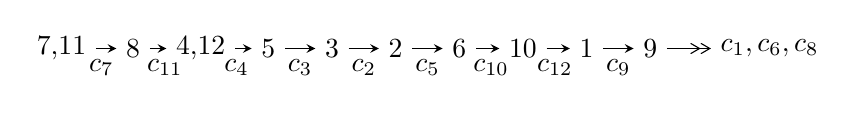
\begin{tikzpicture}[x=23pt, y=7pt]
	% node
	\node (A0) at (-1/8, 0) {7,11};
	\node (A1) at (1, 0) {8};
	\node (A2) at (33/16, 0) {4,12};
	\node (A3) at (25/8, 0) {5};
	\node (A4) at (33/8, 0) {3};
	\node (A5) at (41/8, 0) {2};
	\node (A6) at (49/8, 0) {6};
	\node (A7) at (57/8, 0) {10};
	\node (A8) at (65/8, 0) {1};
	\node (A9) at (73/8, 0) {9};
	\node (C1) at (1/2, -1) {$c_{7}$};
	\node (C2) at (3/2, -1) {$c_{11}$};
	\node (C3) at (21/8, -1) {$c_{4}$};
	\node (C4) at (29/8, -1) {$c_{3}$};
	\node (C5) at (37/8, -1) {$c_{2}$};
	\node (C6) at (45/8, -1) {$c_{5}$};
	\node (C7) at (53/8, -1) {$c_{10}$};
	\node (C8) at (61/8, -1) {$c_{12}$};
	\node (C9) at (69/8, -1) {$c_{9}$};
	\node (A10) at (11, 0) {$c_{1},c_{6},c_{8}$};

	% edge
	\draw[->,>=stealth]	
	(A0) edge (A1) (A1) edge (A2) (A2) edge (A3) (A3) edge (A4) (A4) edge (A5) (A5) edge (A6) (A6) edge (A7) (A7) edge (A8) (A8) edge (A9) ;
	\draw[->>,>={angle 60}]	
	(A9) edge (A10);
\end{tikzpicture} \\ 

\end{tabular} \\

\footnotetext{
The image of knot diagram is generated by the software ``\textbf{Draw programme}" developed by Andrew Bartholomew(\url{http://www.layer8.co.uk/maths/draw/index.htm\#Running-draw}), where we modified some parts for our purpose(\url{https://github.com/CATsTAILs/LinksPainter}).
}\phantom \\ \newline 
\centering \textbf{Ideals for irreducible components\footnotemark of $X_{\text{par}}$} 
 
\begin{align*}
I^u_{1}&=\langle 
-1.28050\times10^{86} u^{56}+4.68989\times10^{86} u^{55}+\cdots+2.10970\times10^{86} b+1.03141\times10^{87},\\
\phantom{I^u_{1}}&\phantom{= \langle  }-3.61697\times10^{87} u^{56}+1.86009\times10^{88} u^{55}+\cdots+4.43037\times10^{87} a-5.59465\times10^{88},\\
\phantom{I^u_{1}}&\phantom{= \langle  }u^{57}-4 u^{56}+\cdots-62 u-21\rangle \\
I^u_{2}&=\langle 
-15113 u^{17}-4096 u^{16}+\cdots+48267 b+50891,\;-57716 u^{17}-93541 u^{16}+\cdots+48267 a-66022,\\
\phantom{I^u_{2}}&\phantom{= \langle  }u^{18}+u^{17}+\cdots-2 u+1\rangle \\
\\
\end{align*}
\raggedright * 2 irreducible components of $\dim_{\mathbb{C}}=0$, with total 75 representations.\\
\footnotetext{All coefficients of polynomials are rational numbers. But the coefficients are sometimes approximated in decimal forms when there is not enough margin.}
\newpage
\renewcommand{\arraystretch}{1}
\centering \section*{I. $I^u_{1}= \langle -1.28\times10^{86} u^{56}+4.69\times10^{86} u^{55}+\cdots+2.11\times10^{86} b+1.03\times10^{87},\;-3.62\times10^{87} u^{56}+1.86\times10^{88} u^{55}+\cdots+4.43\times10^{87} a-5.59\times10^{88},\;u^{57}-4 u^{56}+\cdots-62 u-21 \rangle$}
\flushleft \textbf{(i) Arc colorings}\\
\begin{tabular}{m{7pt} m{180pt} m{7pt} m{180pt} }
\flushright $a_{7}=$&$\begin{pmatrix}1\\0\end{pmatrix}$ \\
\flushright $a_{11}=$&$\begin{pmatrix}0\\u\end{pmatrix}$ \\
\flushright $a_{8}=$&$\begin{pmatrix}1\\u^2\end{pmatrix}$ \\
\flushright $a_{4}=$&$\begin{pmatrix}0.816403 u^{56}-4.19849 u^{55}+\cdots+20.7488 u+12.6279\\0.606959 u^{56}-2.22301 u^{55}+\cdots-20.5606 u-4.88890\end{pmatrix}$ \\
\flushright $a_{12}=$&$\begin{pmatrix}- u\\u\end{pmatrix}$ \\
\flushright $a_{5}=$&$\begin{pmatrix}2.30955 u^{56}-11.2943 u^{55}+\cdots+35.9973 u+27.9170\\-0.886184 u^{56}+4.87279 u^{55}+\cdots-35.8091 u-20.1780\end{pmatrix}$ \\
\flushright $a_{3}=$&$\begin{pmatrix}1.99634 u^{56}-9.90547 u^{55}+\cdots+40.8820 u+27.3294\\-0.548286 u^{56}+3.70956 u^{55}+\cdots-56.9911 u-25.6210\end{pmatrix}$ \\
\flushright $a_{2}=$&$\begin{pmatrix}3.51044 u^{56}-14.4661 u^{55}+\cdots-81.7519 u-6.53532\\-2.08388 u^{56}+9.47088 u^{55}+\cdots+4.37789 u-13.5178\end{pmatrix}$ \\
\flushright $a_{6}=$&$\begin{pmatrix}1.97921 u^{56}-6.06505 u^{55}+\cdots-142.339 u-41.3394\\-1.76709 u^{56}+5.94502 u^{55}+\cdots+103.790 u+27.5904\end{pmatrix}$ \\
\flushright $a_{10}=$&$\begin{pmatrix}-1.72233 u^{56}+5.91243 u^{55}+\cdots+107.267 u+26.4979\\1.60637 u^{56}-5.58082 u^{55}+\cdots-93.6083 u-22.6130\end{pmatrix}$ \\
\flushright $a_{1}=$&$\begin{pmatrix}2.28317 u^{56}-6.62101 u^{55}+\cdots-179.695 u-51.6320\\-1.95007 u^{56}+6.01101 u^{55}+\cdots+139.623 u+39.1357\end{pmatrix}$ \\
\flushright $a_{9}=$&$\begin{pmatrix}0.693372 u^{56}-3.19613 u^{55}+\cdots-2.95802 u+4.39385\\0.216527 u^{56}-0.0576321 u^{55}+\cdots-40.4916 u-13.8044\end{pmatrix}$\\&\end{tabular}
\flushleft \textbf{(ii) Obstruction class $= -1$}\\~\\
\flushleft \textbf{(iii) Cusp Shapes $= -2.42071 u^{56}+9.29216 u^{55}+\cdots+95.3134 u+10.7280$}\\~\\
\newpage\renewcommand{\arraystretch}{1}
\flushleft \textbf{(iv) u-Polynomials at the component}\newline \\
\begin{tabular}{m{50pt}|m{274pt}}
Crossings & \hspace{64pt}u-Polynomials at each crossing \\
\hline $$\begin{aligned}c_{1}\end{aligned}$$&$\begin{aligned}
&u^{57}+75 u^{56}+\cdots-178 u-1
\end{aligned}$\\
\hline $$\begin{aligned}c_{2},c_{5}\end{aligned}$$&$\begin{aligned}
&u^{57}- u^{56}+\cdots-16 u+1
\end{aligned}$\\
\hline $$\begin{aligned}c_{3},c_{8}\end{aligned}$$&$\begin{aligned}
&u^{57}- u^{56}+\cdots-493 u+451
\end{aligned}$\\
\hline $$\begin{aligned}c_{4}\end{aligned}$$&$\begin{aligned}
&u^{57}+3 u^{56}+\cdots-7 u+3
\end{aligned}$\\
\hline $$\begin{aligned}c_{6}\end{aligned}$$&$\begin{aligned}
&u^{57}+u^{56}+\cdots+117087 u+163159
\end{aligned}$\\
\hline $$\begin{aligned}c_{7},c_{11}\end{aligned}$$&$\begin{aligned}
&u^{57}+4 u^{56}+\cdots-62 u+21
\end{aligned}$\\
\hline $$\begin{aligned}c_{9}\end{aligned}$$&$\begin{aligned}
&u^{57}-2 u^{56}+\cdots+1465 u+32979
\end{aligned}$\\
\hline $$\begin{aligned}c_{10}\end{aligned}$$&$\begin{aligned}
&u^{57}+7 u^{55}+\cdots+397 u+97
\end{aligned}$\\
\hline $$\begin{aligned}c_{12}\end{aligned}$$&$\begin{aligned}
&u^{57}-14 u^{56}+\cdots+669 u+151
\end{aligned}$\\
\hline
\end{tabular}\\~\\
\newpage\renewcommand{\arraystretch}{1}
\flushleft \textbf{(v) Riley Polynomials at the component}\newline \\
\begin{tabular}{m{50pt}|m{274pt}}
Crossings & \hspace{64pt}Riley Polynomials at each crossing \\
\hline $$\begin{aligned}c_{1}\end{aligned}$$&$\begin{aligned}
&y^{57}-177 y^{56}+\cdots+14174 y-1
\end{aligned}$\\
\hline $$\begin{aligned}c_{2},c_{5}\end{aligned}$$&$\begin{aligned}
&y^{57}+75 y^{56}+\cdots-178 y-1
\end{aligned}$\\
\hline $$\begin{aligned}c_{3},c_{8}\end{aligned}$$&$\begin{aligned}
&y^{57}+31 y^{56}+\cdots-4225459 y-203401
\end{aligned}$\\
\hline $$\begin{aligned}c_{4}\end{aligned}$$&$\begin{aligned}
&y^{57}-9 y^{56}+\cdots+91 y-9
\end{aligned}$\\
\hline $$\begin{aligned}c_{6}\end{aligned}$$&$\begin{aligned}
&y^{57}+107 y^{56}+\cdots-82651034559 y-26620859281
\end{aligned}$\\
\hline $$\begin{aligned}c_{7},c_{11}\end{aligned}$$&$\begin{aligned}
&y^{57}+44 y^{56}+\cdots-6698 y-441
\end{aligned}$\\
\hline $$\begin{aligned}c_{9}\end{aligned}$$&$\begin{aligned}
&y^{57}+78 y^{56}+\cdots+20424721765 y-1087614441
\end{aligned}$\\
\hline $$\begin{aligned}c_{10}\end{aligned}$$&$\begin{aligned}
&y^{57}+14 y^{56}+\cdots-194501 y-9409
\end{aligned}$\\
\hline $$\begin{aligned}c_{12}\end{aligned}$$&$\begin{aligned}
&y^{57}-40 y^{56}+\cdots+3746609 y-22801
\end{aligned}$\\
\hline
\end{tabular}\\~\\
\newpage\flushleft \textbf{(vi) Complex Volumes and Cusp Shapes}
$$\begin{array}{c|c|c}  
\text{Solutions to }I^u_{1}& \I (\text{vol} + \sqrt{-1}CS) & \text{Cusp shape}\\
 \hline 
\begin{aligned}
u &= \phantom{-}0.590251 + 0.816756 I \\
a &= -0.317194 - 0.867682 I \\
b &= \phantom{-}0.851232 + 0.408615 I\end{aligned}
 & -0.92370 - 2.38461 I & -6.78715 - 4.77142 I \\ \hline\begin{aligned}
u &= \phantom{-}0.590251 - 0.816756 I \\
a &= -0.317194 + 0.867682 I \\
b &= \phantom{-}0.851232 - 0.408615 I\end{aligned}
 & -0.92370 + 2.38461 I & -6.78715 + 4.77142 I \\ \hline\begin{aligned}
u &= \phantom{-}0.386358 + 0.881902 I \\
a &= -1.004400 - 0.119570 I \\
b &= \phantom{-}1.290360 - 0.133007 I\end{aligned}
 & -0.66188 - 1.95236 I & -7.77812 + 3.23861 I \\ \hline\begin{aligned}
u &= \phantom{-}0.386358 - 0.881902 I \\
a &= -1.004400 + 0.119570 I \\
b &= \phantom{-}1.290360 + 0.133007 I\end{aligned}
 & -0.66188 + 1.95236 I & -7.77812 - 3.23861 I \\ \hline\begin{aligned}
u &= -0.113138 + 1.043540 I \\
a &= \phantom{-}0.010650 + 1.316020 I \\
b &= \phantom{-}0.398262 - 0.207554 I\end{aligned}
 & \phantom{-}1.52820 + 3.04852 I & -2.09627 - 4.89869 I \\ \hline\begin{aligned}
u &= -0.113138 - 1.043540 I \\
a &= \phantom{-}0.010650 - 1.316020 I \\
b &= \phantom{-}0.398262 + 0.207554 I\end{aligned}
 & \phantom{-}1.52820 - 3.04852 I & -2.09627 + 4.89869 I \\ \hline\begin{aligned}
u &= -0.054065 + 1.061160 I \\
a &= -0.673299 - 0.339769 I \\
b &= \phantom{-}1.23289 - 1.36328 I\end{aligned}
 & \phantom{-}4.35464 + 0.41270 I & \phantom{-0.000000 -}0. + 2.93923 I \\ \hline\begin{aligned}
u &= -0.054065 - 1.061160 I \\
a &= -0.673299 + 0.339769 I \\
b &= \phantom{-}1.23289 + 1.36328 I\end{aligned}
 & \phantom{-}4.35464 - 0.41270 I & \phantom{-0.000000 } 0. - 2.93923 I \\ \hline\begin{aligned}
u &= -0.135302 + 1.081390 I \\
a &= \phantom{-}0.86661 - 2.26881 I \\
b &= -1.29656 + 1.44749 I\end{aligned}
 & -7.16107 + 4.13510 I & \phantom{-0.000000 } 0 \\ \hline\begin{aligned}
u &= -0.135302 - 1.081390 I \\
a &= \phantom{-}0.86661 + 2.26881 I \\
b &= -1.29656 - 1.44749 I\end{aligned}
 & -7.16107 - 4.13510 I & \phantom{-0.000000 } 0\\
 \hline 
 \end{array}$$\newpage$$\begin{array}{c|c|c}  
\text{Solutions to }I^u_{1}& \I (\text{vol} + \sqrt{-1}CS) & \text{Cusp shape}\\
 \hline 
\begin{aligned}
u &= \phantom{-}0.563215 + 0.991464 I \\
a &= \phantom{-}0.95892 + 1.31146 I \\
b &= -1.68040 - 0.81381 I\end{aligned}
 & -6.73101 - 1.00486 I & \phantom{-0.000000 } 0 \\ \hline\begin{aligned}
u &= \phantom{-}0.563215 - 0.991464 I \\
a &= \phantom{-}0.95892 - 1.31146 I \\
b &= -1.68040 + 0.81381 I\end{aligned}
 & -6.73101 + 1.00486 I & \phantom{-0.000000 } 0 \\ \hline\begin{aligned}
u &= \phantom{-}0.076850 + 1.138320 I \\
a &= \phantom{-}0.774845 - 0.307436 I \\
b &= -1.84851 + 0.66895 I\end{aligned}
 & \phantom{-}2.81588 - 1.84751 I & \phantom{-0.000000 } 0 \\ \hline\begin{aligned}
u &= \phantom{-}0.076850 - 1.138320 I \\
a &= \phantom{-}0.774845 + 0.307436 I \\
b &= -1.84851 - 0.66895 I\end{aligned}
 & \phantom{-}2.81588 + 1.84751 I & \phantom{-0.000000 } 0 \\ \hline\begin{aligned}
u &= -0.210776 + 1.134080 I \\
a &= -0.376842 + 0.250683 I \\
b &= \phantom{-}1.62012 + 0.80598 I\end{aligned}
 & \phantom{-}1.73829 + 3.89054 I & \phantom{-0.000000 } 0 \\ \hline\begin{aligned}
u &= -0.210776 - 1.134080 I \\
a &= -0.376842 - 0.250683 I \\
b &= \phantom{-}1.62012 - 0.80598 I\end{aligned}
 & \phantom{-}1.73829 - 3.89054 I & \phantom{-0.000000 } 0 \\ \hline\begin{aligned}
u &= -0.758593 + 0.355885 I \\
a &= \phantom{-}0.642976 + 0.011129 I \\
b &= \phantom{-}0.033112 + 0.742505 I\end{aligned}
 & -0.664386 - 0.689297 I & -6.71036 - 0.11936 I \\ \hline\begin{aligned}
u &= -0.758593 - 0.355885 I \\
a &= \phantom{-}0.642976 - 0.011129 I \\
b &= \phantom{-}0.033112 - 0.742505 I\end{aligned}
 & -0.664386 + 0.689297 I & -6.71036 + 0.11936 I \\ \hline\begin{aligned}
u &= -0.778647 + 0.303273 I \\
a &= -1.16942 - 0.93924 I \\
b &= \phantom{-}0.147887 - 0.411465 I\end{aligned}
 & -12.42110 - 2.33478 I & -9.22240 + 0.68624 I \\ \hline\begin{aligned}
u &= -0.778647 - 0.303273 I \\
a &= -1.16942 + 0.93924 I \\
b &= \phantom{-}0.147887 + 0.411465 I\end{aligned}
 & -12.42110 + 2.33478 I & -9.22240 - 0.68624 I\\
 \hline 
 \end{array}$$\newpage$$\begin{array}{c|c|c}  
\text{Solutions to }I^u_{1}& \I (\text{vol} + \sqrt{-1}CS) & \text{Cusp shape}\\
 \hline 
\begin{aligned}
u &= \phantom{-}1.179050 + 0.038215 I \\
a &= -0.705861 - 0.743030 I \\
b &= -0.185989 + 0.148446 I\end{aligned}
 & -9.92606 - 9.08178 I & \phantom{-0.000000 } 0 \\ \hline\begin{aligned}
u &= \phantom{-}1.179050 - 0.038215 I \\
a &= -0.705861 + 0.743030 I \\
b &= -0.185989 - 0.148446 I\end{aligned}
 & -9.92606 + 9.08178 I & \phantom{-0.000000 } 0 \\ \hline\begin{aligned}
u &= -0.413385 + 1.107260 I \\
a &= \phantom{-}0.654823 + 0.404099 I \\
b &= -2.11452 - 1.09525 I\end{aligned}
 & -9.95724 + 6.72104 I & \phantom{-0.000000 } 0 \\ \hline\begin{aligned}
u &= -0.413385 - 1.107260 I \\
a &= \phantom{-}0.654823 - 0.404099 I \\
b &= -2.11452 + 1.09525 I\end{aligned}
 & -9.95724 - 6.72104 I & \phantom{-0.000000 } 0 \\ \hline\begin{aligned}
u &= \phantom{-}0.039564 + 1.190590 I \\
a &= \phantom{-}0.613863 - 0.424692 I \\
b &= -1.80875 - 0.41422 I\end{aligned}
 & \phantom{-}3.76883 - 1.63591 I & \phantom{-0.000000 } 0 \\ \hline\begin{aligned}
u &= \phantom{-}0.039564 - 1.190590 I \\
a &= \phantom{-}0.613863 + 0.424692 I \\
b &= -1.80875 + 0.41422 I\end{aligned}
 & \phantom{-}3.76883 + 1.63591 I & \phantom{-0.000000 } 0 \\ \hline\begin{aligned}
u &= \phantom{-}1.218100 + 0.242266 I \\
a &= \phantom{-}0.507438 + 0.284538 I \\
b &= \phantom{-}0.1171880 - 0.0218347 I\end{aligned}
 & -1.64373 - 3.94719 I & \phantom{-0.000000 } 0 \\ \hline\begin{aligned}
u &= \phantom{-}1.218100 - 0.242266 I \\
a &= \phantom{-}0.507438 - 0.284538 I \\
b &= \phantom{-}0.1171880 + 0.0218347 I\end{aligned}
 & -1.64373 + 3.94719 I & \phantom{-0.000000 } 0 \\ \hline\begin{aligned}
u &= \phantom{-}0.254408 + 1.227690 I \\
a &= -0.823428 + 0.385148 I \\
b &= \phantom{-}2.00617 + 0.66223 I\end{aligned}
 & -4.08404 - 6.16672 I & \phantom{-0.000000 } 0 \\ \hline\begin{aligned}
u &= \phantom{-}0.254408 - 1.227690 I \\
a &= -0.823428 - 0.385148 I \\
b &= \phantom{-}2.00617 - 0.66223 I\end{aligned}
 & -4.08404 + 6.16672 I & \phantom{-0.000000 } 0\\
 \hline 
 \end{array}$$\newpage$$\begin{array}{c|c|c}  
\text{Solutions to }I^u_{1}& \I (\text{vol} + \sqrt{-1}CS) & \text{Cusp shape}\\
 \hline 
\begin{aligned}
u &= -0.727598 + 0.137352 I \\
a &= -0.875509 + 0.961139 I \\
b &= -0.173507 - 0.506822 I\end{aligned}
 & \phantom{-}2.46442 + 1.93449 I & \phantom{-}2.24278 - 3.17004 I \\ \hline\begin{aligned}
u &= -0.727598 - 0.137352 I \\
a &= -0.875509 - 0.961139 I \\
b &= -0.173507 + 0.506822 I\end{aligned}
 & \phantom{-}2.46442 - 1.93449 I & \phantom{-}2.24278 + 3.17004 I \\ \hline\begin{aligned}
u &= -0.392456 + 1.219230 I \\
a &= -1.257630 - 0.153845 I \\
b &= \phantom{-}2.26538 + 0.66065 I\end{aligned}
 & \phantom{-}1.90935 + 6.56503 I & \phantom{-0.000000 } 0 \\ \hline\begin{aligned}
u &= -0.392456 - 1.219230 I \\
a &= -1.257630 + 0.153845 I \\
b &= \phantom{-}2.26538 - 0.66065 I\end{aligned}
 & \phantom{-}1.90935 - 6.56503 I & \phantom{-0.000000 } 0 \\ \hline\begin{aligned}
u &= \phantom{-}0.010268 + 0.689208 I \\
a &= \phantom{-}2.53605 + 1.22720 I \\
b &= -2.04707 - 1.45230 I\end{aligned}
 & -8.64761 - 3.10440 I & -7.56449 - 2.31310 I \\ \hline\begin{aligned}
u &= \phantom{-}0.010268 - 0.689208 I \\
a &= \phantom{-}2.53605 - 1.22720 I \\
b &= -2.04707 + 1.45230 I\end{aligned}
 & -8.64761 + 3.10440 I & -7.56449 + 2.31310 I \\ \hline\begin{aligned}
u &= -0.618158 + 0.162095 I \\
a &= \phantom{-}0.81252 + 1.47630 I \\
b &= \phantom{-}0.266464 - 0.032773 I\end{aligned}
 & -1.35954 - 2.62834 I & -9.01490 + 3.76676 I \\ \hline\begin{aligned}
u &= -0.618158 - 0.162095 I \\
a &= \phantom{-}0.81252 - 1.47630 I \\
b &= \phantom{-}0.266464 + 0.032773 I\end{aligned}
 & -1.35954 + 2.62834 I & -9.01490 - 3.76676 I \\ \hline\begin{aligned}
u &= -0.427624 + 1.306800 I \\
a &= \phantom{-}1.316570 + 0.287086 I \\
b &= -2.05986 - 0.58492 I\end{aligned}
 & \phantom{-}6.77585 + 6.29606 I & \phantom{-0.000000 } 0 \\ \hline\begin{aligned}
u &= -0.427624 - 1.306800 I \\
a &= \phantom{-}1.316570 - 0.287086 I \\
b &= -2.05986 + 0.58492 I\end{aligned}
 & \phantom{-}6.77585 - 6.29606 I & \phantom{-0.000000 } 0\\
 \hline 
 \end{array}$$\newpage$$\begin{array}{c|c|c}  
\text{Solutions to }I^u_{1}& \I (\text{vol} + \sqrt{-1}CS) & \text{Cusp shape}\\
 \hline 
\begin{aligned}
u &= \phantom{-}0.540765 + 0.298006 I \\
a &= \phantom{-}1.21617 + 1.81557 I \\
b &= -1.173460 - 0.320334 I\end{aligned}
 & -8.36689 - 3.37214 I & -6.78658 + 1.79216 I \\ \hline\begin{aligned}
u &= \phantom{-}0.540765 - 0.298006 I \\
a &= \phantom{-}1.21617 - 1.81557 I \\
b &= -1.173460 + 0.320334 I\end{aligned}
 & -8.36689 + 3.37214 I & -6.78658 - 1.79216 I \\ \hline\begin{aligned}
u &= \phantom{-}0.565613\phantom{ +0.000000I} \\
a &= -1.21094\phantom{ +0.000000I} \\
b &= \phantom{-}0.0986015\phantom{ +0.000000I}\end{aligned}
 & -1.05400\phantom{ +0.000000I} & -9.48580\phantom{ +0.000000I} \\ \hline\begin{aligned}
u &= \phantom{-}0.55473 + 1.39062 I \\
a &= \phantom{-}1.170690 - 0.365984 I \\
b &= -2.11486 + 0.87983 I\end{aligned}
 & -5.4571 - 15.1423 I & \phantom{-0.000000 } 0 \\ \hline\begin{aligned}
u &= \phantom{-}0.55473 - 1.39062 I \\
a &= \phantom{-}1.170690 + 0.365984 I \\
b &= -2.11486 - 0.87983 I\end{aligned}
 & -5.4571 + 15.1423 I & \phantom{-0.000000 } 0 \\ \hline\begin{aligned}
u &= \phantom{-}0.38131 + 1.45291 I \\
a &= \phantom{-}0.713409 - 0.306037 I \\
b &= -1.46415 + 0.57342 I\end{aligned}
 & \phantom{-}4.12609 - 3.19316 I & \phantom{-0.000000 } 0 \\ \hline\begin{aligned}
u &= \phantom{-}0.38131 - 1.45291 I \\
a &= \phantom{-}0.713409 + 0.306037 I \\
b &= -1.46415 - 0.57342 I\end{aligned}
 & \phantom{-}4.12609 + 3.19316 I & \phantom{-0.000000 } 0 \\ \hline\begin{aligned}
u &= \phantom{-}0.51803 + 1.42333 I \\
a &= -0.910861 + 0.309333 I \\
b &= \phantom{-}1.80097 - 0.72599 I\end{aligned}
 & \phantom{-}3.42580 - 9.91933 I & \phantom{-0.000000 } 0 \\ \hline\begin{aligned}
u &= \phantom{-}0.51803 - 1.42333 I \\
a &= -0.910861 - 0.309333 I \\
b &= \phantom{-}1.80097 + 0.72599 I\end{aligned}
 & \phantom{-}3.42580 + 9.91933 I & \phantom{-0.000000 } 0 \\ \hline\begin{aligned}
u &= -0.55233 + 1.42025 I \\
a &= -0.872585 - 0.293555 I \\
b &= \phantom{-}1.270760 + 0.462620 I\end{aligned}
 & \phantom{-}5.06769 + 4.73436 I & \phantom{-0.000000 } 0\\
 \hline 
 \end{array}$$\newpage$$\begin{array}{c|c|c}  
\text{Solutions to }I^u_{1}& \I (\text{vol} + \sqrt{-1}CS) & \text{Cusp shape}\\
 \hline 
\begin{aligned}
u &= -0.55233 - 1.42025 I \\
a &= -0.872585 + 0.293555 I \\
b &= \phantom{-}1.270760 - 0.462620 I\end{aligned}
 & \phantom{-}5.06769 - 4.73436 I & \phantom{-0.000000 } 0 \\ \hline\begin{aligned}
u &= -0.150198 + 0.275358 I \\
a &= -1.53020 + 0.49740 I \\
b &= \phantom{-}0.487442 + 0.712451 I\end{aligned}
 & -0.19079 - 1.54094 I & -2.12423 + 2.96705 I \\ \hline\begin{aligned}
u &= -0.150198 - 0.275358 I \\
a &= -1.53020 - 0.49740 I \\
b &= \phantom{-}0.487442 - 0.712451 I\end{aligned}
 & -0.19079 + 1.54094 I & -2.12423 - 2.96705 I \\ \hline\begin{aligned}
u &= \phantom{-}0.84030 + 1.60146 I \\
a &= -0.248588 - 0.091885 I \\
b &= \phantom{-}0.286209 + 0.417616 I\end{aligned}
 & -5.54252 + 2.13223 I & \phantom{-0.000000 } 0 \\ \hline\begin{aligned}
u &= \phantom{-}0.84030 - 1.60146 I \\
a &= -0.248588 + 0.091885 I \\
b &= \phantom{-}0.286209 - 0.417616 I\end{aligned}
 & -5.54252 - 2.13223 I & \phantom{-0.000000 } 0 \\ \hline\begin{aligned}
u &= -0.10374 + 1.81764 I \\
a &= -0.162358 + 0.545197 I \\
b &= \phantom{-}0.343904 - 0.804109 I\end{aligned}
 & -5.52482 + 1.18551 I & \phantom{-0.000000 } 0 \\ \hline\begin{aligned}
u &= -0.10374 - 1.81764 I \\
a &= -0.162358 - 0.545197 I \\
b &= \phantom{-}0.343904 + 0.804109 I\end{aligned}
 & -5.52482 - 1.18551 I & \phantom{-0.000000 } 0\\
 \hline 
 \end{array}$$\newpage\newpage\renewcommand{\arraystretch}{1}
\centering \section*{II. $I^u_{2}= \langle -15113 u^{17}-4096 u^{16}+\cdots+48267 b+50891,\;-57716 u^{17}-93541 u^{16}+\cdots+48267 a-66022,\;u^{18}+u^{17}+\cdots-2 u+1 \rangle$}
\flushleft \textbf{(i) Arc colorings}\\
\begin{tabular}{m{7pt} m{180pt} m{7pt} m{180pt} }
\flushright $a_{7}=$&$\begin{pmatrix}1\\0\end{pmatrix}$ \\
\flushright $a_{11}=$&$\begin{pmatrix}0\\u\end{pmatrix}$ \\
\flushright $a_{8}=$&$\begin{pmatrix}1\\u^2\end{pmatrix}$ \\
\flushright $a_{4}=$&$\begin{pmatrix}1.19577 u^{17}+1.93799 u^{16}+\cdots+10.2808 u+1.36785\\0.313112 u^{17}+0.0848613 u^{16}+\cdots+4.67019 u-1.05436\end{pmatrix}$ \\
\flushright $a_{12}=$&$\begin{pmatrix}- u\\u\end{pmatrix}$ \\
\flushright $a_{5}=$&$\begin{pmatrix}1.18369 u^{17}+2.40398 u^{16}+\cdots+10.7617 u+1.88182\\0.325191 u^{17}-0.381130 u^{16}+\cdots+4.18926 u-1.56834\end{pmatrix}$ \\
\flushright $a_{3}=$&$\begin{pmatrix}1.31137 u^{17}+2.05938 u^{16}+\cdots+14.6623 u+1.05571\\0.463401 u^{17}+0.142665 u^{16}+\cdots+4.56614 u-1.06014\end{pmatrix}$ \\
\flushright $a_{2}=$&$\begin{pmatrix}2.41569 u^{17}+2.94400 u^{16}+\cdots+11.5997 u+3.70775\\-1.22525 u^{17}-1.72683 u^{16}+\cdots+2.12120 u+0.246877\end{pmatrix}$ \\
\flushright $a_{6}=$&$\begin{pmatrix}-1.10968 u^{17}-2.46319 u^{16}+\cdots-3.71177 u+1.43736\\-1.01954 u^{17}+0.0710630 u^{16}+\cdots-5.12433 u+2.98573\end{pmatrix}$ \\
\flushright $a_{10}=$&$\begin{pmatrix}-1.26256 u^{17}-0.630348 u^{16}+\cdots-10.0123 u-0.143058\\1.38287 u^{17}+0.606315 u^{16}+\cdots+3.73659 u-2.21655\end{pmatrix}$ \\
\flushright $a_{1}=$&$\begin{pmatrix}0.336669 u^{17}-0.784490 u^{16}+\cdots-1.40154 u+0.205689\\-1.59461 u^{17}-0.706777 u^{16}+\cdots-4.69698 u+2.60903\end{pmatrix}$ \\
\flushright $a_{9}=$&$\begin{pmatrix}1.58433 u^{17}+0.984876 u^{16}+\cdots+9.50751 u-3.95906\\-0.464023 u^{17}-1.00891 u^{16}+\cdots+0.216753 u-1.40054\end{pmatrix}$\\&\end{tabular}
\flushleft \textbf{(ii) Obstruction class $= 1$}\\~\\
\flushleft \textbf{(iii) Cusp Shapes $= -\frac{90767}{16089} u^{17}-\frac{105175}{16089} u^{16}+\cdots-\frac{268616}{16089} u-\frac{63094}{16089}$}\\~\\
\newpage\renewcommand{\arraystretch}{1}
\flushleft \textbf{(iv) u-Polynomials at the component}\newline \\
\begin{tabular}{m{50pt}|m{274pt}}
Crossings & \hspace{64pt}u-Polynomials at each crossing \\
\hline $$\begin{aligned}c_{1}\end{aligned}$$&$\begin{aligned}
&u^{18}-20 u^{17}+\cdots-74 u+9
\end{aligned}$\\
\hline $$\begin{aligned}c_{2}\end{aligned}$$&$\begin{aligned}
&u^{18}+2 u^{17}+\cdots+10 u+3
\end{aligned}$\\
\hline $$\begin{aligned}c_{3}\end{aligned}$$&$\begin{aligned}
&u^{18}+8 u^{16}+\cdots-3 u+9
\end{aligned}$\\
\hline $$\begin{aligned}c_{4}\end{aligned}$$&$\begin{aligned}
&u^{18}-2 u^{17}+\cdots-5 u+1
\end{aligned}$\\
\hline $$\begin{aligned}c_{5}\end{aligned}$$&$\begin{aligned}
&u^{18}-2 u^{17}+\cdots-10 u+3
\end{aligned}$\\
\hline $$\begin{aligned}c_{6}\end{aligned}$$&$\begin{aligned}
&u^{18}-2 u^{17}+\cdots-5 u+3
\end{aligned}$\\
\hline $$\begin{aligned}c_{7}\end{aligned}$$&$\begin{aligned}
&u^{18}+u^{17}+\cdots-2 u+1
\end{aligned}$\\
\hline $$\begin{aligned}c_{8}\end{aligned}$$&$\begin{aligned}
&u^{18}+8 u^{16}+\cdots+3 u+9
\end{aligned}$\\
\hline $$\begin{aligned}c_{9}\end{aligned}$$&$\begin{aligned}
&u^{18}+u^{17}+\cdots+u+1
\end{aligned}$\\
\hline $$\begin{aligned}c_{10}\end{aligned}$$&$\begin{aligned}
&u^{18}+u^{17}+\cdots-7 u+3
\end{aligned}$\\
\hline $$\begin{aligned}c_{11}\end{aligned}$$&$\begin{aligned}
&u^{18}- u^{17}+\cdots+2 u+1
\end{aligned}$\\
\hline $$\begin{aligned}c_{12}\end{aligned}$$&$\begin{aligned}
&u^{18}-5 u^{17}+\cdots+15 u+9
\end{aligned}$\\
\hline
\end{tabular}\\~\\
\newpage\renewcommand{\arraystretch}{1}
\flushleft \textbf{(v) Riley Polynomials at the component}\newline \\
\begin{tabular}{m{50pt}|m{274pt}}
Crossings & \hspace{64pt}Riley Polynomials at each crossing \\
\hline $$\begin{aligned}c_{1}\end{aligned}$$&$\begin{aligned}
&y^{18}-36 y^{17}+\cdots+1454 y+81
\end{aligned}$\\
\hline $$\begin{aligned}c_{2},c_{5}\end{aligned}$$&$\begin{aligned}
&y^{18}+20 y^{17}+\cdots+74 y+9
\end{aligned}$\\
\hline $$\begin{aligned}c_{3},c_{8}\end{aligned}$$&$\begin{aligned}
&y^{18}+16 y^{17}+\cdots+1035 y+81
\end{aligned}$\\
\hline $$\begin{aligned}c_{4}\end{aligned}$$&$\begin{aligned}
&y^{18}-4 y^{17}+\cdots-7 y+1
\end{aligned}$\\
\hline $$\begin{aligned}c_{6}\end{aligned}$$&$\begin{aligned}
&y^{18}+20 y^{17}+\cdots+131 y+9
\end{aligned}$\\
\hline $$\begin{aligned}c_{7},c_{11}\end{aligned}$$&$\begin{aligned}
&y^{18}+17 y^{17}+\cdots+22 y+1
\end{aligned}$\\
\hline $$\begin{aligned}c_{9}\end{aligned}$$&$\begin{aligned}
&y^{18}+11 y^{17}+\cdots-9 y+1
\end{aligned}$\\
\hline $$\begin{aligned}c_{10}\end{aligned}$$&$\begin{aligned}
&y^{18}+7 y^{17}+\cdots+53 y+9
\end{aligned}$\\
\hline $$\begin{aligned}c_{12}\end{aligned}$$&$\begin{aligned}
&y^{18}-15 y^{17}+\cdots+495 y+81
\end{aligned}$\\
\hline
\end{tabular}\\~\\
\newpage\flushleft \textbf{(vi) Complex Volumes and Cusp Shapes}
$$\begin{array}{c|c|c}  
\text{Solutions to }I^u_{2}& \I (\text{vol} + \sqrt{-1}CS) & \text{Cusp shape}\\
 \hline 
\begin{aligned}
u &= -0.955128 + 0.028468 I \\
a &= -0.470624 + 0.928452 I \\
b &= -0.378740 - 0.352785 I\end{aligned}
 & \phantom{-}1.45067 + 2.23926 I & -5.74852 - 4.22019 I \\ \hline\begin{aligned}
u &= -0.955128 - 0.028468 I \\
a &= -0.470624 - 0.928452 I \\
b &= -0.378740 + 0.352785 I\end{aligned}
 & \phantom{-}1.45067 - 2.23926 I & -5.74852 + 4.22019 I \\ \hline\begin{aligned}
u &= \phantom{-}0.588467 + 0.644672 I \\
a &= \phantom{-}0.004247 + 0.886743 I \\
b &= -0.771830 - 0.597373 I\end{aligned}
 & -0.77892 - 2.83224 I & -2.15898 + 10.71484 I \\ \hline\begin{aligned}
u &= \phantom{-}0.588467 - 0.644672 I \\
a &= \phantom{-}0.004247 - 0.886743 I \\
b &= -0.771830 + 0.597373 I\end{aligned}
 & -0.77892 + 2.83224 I & -2.15898 - 10.71484 I \\ \hline\begin{aligned}
u &= \phantom{-}0.157250 + 1.129630 I \\
a &= \phantom{-}0.747231 + 0.158603 I \\
b &= -2.20016 + 0.80914 I\end{aligned}
 & \phantom{-}2.38693 - 3.66478 I & \phantom{-}3.78363 + 3.00827 I \\ \hline\begin{aligned}
u &= \phantom{-}0.157250 - 1.129630 I \\
a &= \phantom{-}0.747231 - 0.158603 I \\
b &= -2.20016 - 0.80914 I\end{aligned}
 & \phantom{-}2.38693 + 3.66478 I & \phantom{-}3.78363 - 3.00827 I \\ \hline\begin{aligned}
u &= -0.104673 + 1.160730 I \\
a &= -0.526573 - 0.204291 I \\
b &= \phantom{-}1.35939 - 1.31112 I\end{aligned}
 & \phantom{-}4.61635 + 1.06986 I & \phantom{-}5.50666 - 5.36656 I \\ \hline\begin{aligned}
u &= -0.104673 - 1.160730 I \\
a &= -0.526573 + 0.204291 I \\
b &= \phantom{-}1.35939 + 1.31112 I\end{aligned}
 & \phantom{-}4.61635 - 1.06986 I & \phantom{-}5.50666 + 5.36656 I \\ \hline\begin{aligned}
u &= \phantom{-}0.193538 + 0.774845 I \\
a &= -1.28604 - 2.17413 I \\
b &= \phantom{-}2.12934 + 1.50102 I\end{aligned}
 & -8.58566 - 3.82241 I & -7.48775 + 7.44013 I \\ \hline\begin{aligned}
u &= \phantom{-}0.193538 - 0.774845 I \\
a &= -1.28604 + 2.17413 I \\
b &= \phantom{-}2.12934 - 1.50102 I\end{aligned}
 & -8.58566 + 3.82241 I & -7.48775 - 7.44013 I\\
 \hline 
 \end{array}$$\newpage$$\begin{array}{c|c|c}  
\text{Solutions to }I^u_{2}& \I (\text{vol} + \sqrt{-1}CS) & \text{Cusp shape}\\
 \hline 
\begin{aligned}
u &= -0.53247 + 1.34251 I \\
a &= \phantom{-}1.188420 + 0.044021 I \\
b &= -1.97913 - 0.43683 I\end{aligned}
 & \phantom{-}5.61740 + 7.69065 I & -2.00686 - 6.54591 I \\ \hline\begin{aligned}
u &= -0.53247 - 1.34251 I \\
a &= \phantom{-}1.188420 - 0.044021 I \\
b &= -1.97913 + 0.43683 I\end{aligned}
 & \phantom{-}5.61740 - 7.69065 I & -2.00686 + 6.54591 I \\ \hline\begin{aligned}
u &= -0.38473 + 1.43619 I \\
a &= -0.912804 - 0.458239 I \\
b &= \phantom{-}1.56484 + 0.58036 I\end{aligned}
 & \phantom{-}6.11112 + 4.38817 I & \phantom{-}1.91777 - 2.70230 I \\ \hline\begin{aligned}
u &= -0.38473 - 1.43619 I \\
a &= -0.912804 + 0.458239 I \\
b &= \phantom{-}1.56484 - 0.58036 I\end{aligned}
 & \phantom{-}6.11112 - 4.38817 I & \phantom{-}1.91777 + 2.70230 I \\ \hline\begin{aligned}
u &= \phantom{-}0.109990 + 0.279939 I \\
a &= \phantom{-}0.67048 + 2.80242 I \\
b &= -0.062626 + 0.797311 I\end{aligned}
 & -0.15418 + 2.05102 I & -3.58795 - 2.95582 I \\ \hline\begin{aligned}
u &= \phantom{-}0.109990 - 0.279939 I \\
a &= \phantom{-}0.67048 - 2.80242 I \\
b &= -0.062626 - 0.797311 I\end{aligned}
 & -0.15418 - 2.05102 I & -3.58795 + 2.95582 I \\ \hline\begin{aligned}
u &= \phantom{-}0.42776 + 1.69552 I \\
a &= -0.414340 + 0.265180 I \\
b &= \phantom{-}0.338917 - 0.418197 I\end{aligned}
 & -5.72891 + 1.72338 I & -11.71800 - 0.30191 I \\ \hline\begin{aligned}
u &= \phantom{-}0.42776 - 1.69552 I \\
a &= -0.414340 - 0.265180 I \\
b &= \phantom{-}0.338917 + 0.418197 I\end{aligned}
 & -5.72891 - 1.72338 I & -11.71800 + 0.30191 I\\
 \hline 
 \end{array}$$\newpage
\newpage\renewcommand{\arraystretch}{1}
\centering \section*{ III. u-Polynomials}
\begin{tabular}{m{50pt}|m{274pt}}
Crossings & \hspace{64pt}u-Polynomials at each crossing \\
\hline $$\begin{aligned}c_{1}\end{aligned}$$&$\begin{aligned}
&(u^{18}-20 u^{17}+\cdots-74 u+9)(u^{57}+75 u^{56}+\cdots-178 u-1)
\end{aligned}$\\
\hline $$\begin{aligned}c_{2}\end{aligned}$$&$\begin{aligned}
&(u^{18}+2 u^{17}+\cdots+10 u+3)(u^{57}- u^{56}+\cdots-16 u+1)
\end{aligned}$\\
\hline $$\begin{aligned}c_{3}\end{aligned}$$&$\begin{aligned}
&(u^{18}+8 u^{16}+\cdots-3 u+9)(u^{57}- u^{56}+\cdots-493 u+451)
\end{aligned}$\\
\hline $$\begin{aligned}c_{4}\end{aligned}$$&$\begin{aligned}
&(u^{18}-2 u^{17}+\cdots-5 u+1)(u^{57}+3 u^{56}+\cdots-7 u+3)
\end{aligned}$\\
\hline $$\begin{aligned}c_{5}\end{aligned}$$&$\begin{aligned}
&(u^{18}-2 u^{17}+\cdots-10 u+3)(u^{57}- u^{56}+\cdots-16 u+1)
\end{aligned}$\\
\hline $$\begin{aligned}c_{6}\end{aligned}$$&$\begin{aligned}
&(u^{18}-2 u^{17}+\cdots-5 u+3)(u^{57}+u^{56}+\cdots+117087 u+163159)
\end{aligned}$\\
\hline $$\begin{aligned}c_{7}\end{aligned}$$&$\begin{aligned}
&(u^{18}+u^{17}+\cdots-2 u+1)(u^{57}+4 u^{56}+\cdots-62 u+21)
\end{aligned}$\\
\hline $$\begin{aligned}c_{8}\end{aligned}$$&$\begin{aligned}
&(u^{18}+8 u^{16}+\cdots+3 u+9)(u^{57}- u^{56}+\cdots-493 u+451)
\end{aligned}$\\
\hline $$\begin{aligned}c_{9}\end{aligned}$$&$\begin{aligned}
&(u^{18}+u^{17}+\cdots+u+1)(u^{57}-2 u^{56}+\cdots+1465 u+32979)
\end{aligned}$\\
\hline $$\begin{aligned}c_{10}\end{aligned}$$&$\begin{aligned}
&(u^{18}+u^{17}+\cdots-7 u+3)(u^{57}+7 u^{55}+\cdots+397 u+97)
\end{aligned}$\\
\hline $$\begin{aligned}c_{11}\end{aligned}$$&$\begin{aligned}
&(u^{18}- u^{17}+\cdots+2 u+1)(u^{57}+4 u^{56}+\cdots-62 u+21)
\end{aligned}$\\
\hline $$\begin{aligned}c_{12}\end{aligned}$$&$\begin{aligned}
&(u^{18}-5 u^{17}+\cdots+15 u+9)(u^{57}-14 u^{56}+\cdots+669 u+151)
\end{aligned}$\\
\hline
\end{tabular}\newpage\renewcommand{\arraystretch}{1}
\centering \section*{ IV. Riley Polynomials}
\begin{tabular}{m{50pt}|m{274pt}}
Crossings & \hspace{64pt}Riley Polynomials at each crossing \\
\hline $$\begin{aligned}c_{1}\end{aligned}$$&$\begin{aligned}
&(y^{18}-36 y^{17}+\cdots+1454 y+81)(y^{57}-177 y^{56}+\cdots+14174 y-1)
\end{aligned}$\\
\hline $$\begin{aligned}c_{2},c_{5}\end{aligned}$$&$\begin{aligned}
&(y^{18}+20 y^{17}+\cdots+74 y+9)(y^{57}+75 y^{56}+\cdots-178 y-1)
\end{aligned}$\\
\hline $$\begin{aligned}c_{3},c_{8}\end{aligned}$$&$\begin{aligned}
&(y^{18}+16 y^{17}+\cdots+1035 y+81)\\
&\cdot(y^{57}+31 y^{56}+\cdots-4225459 y-203401)
\end{aligned}$\\
\hline $$\begin{aligned}c_{4}\end{aligned}$$&$\begin{aligned}
&(y^{18}-4 y^{17}+\cdots-7 y+1)(y^{57}-9 y^{56}+\cdots+91 y-9)
\end{aligned}$\\
\hline $$\begin{aligned}c_{6}\end{aligned}$$&$\begin{aligned}
&(y^{18}+20 y^{17}+\cdots+131 y+9)\\
&\cdot(y^{57}+107 y^{56}+\cdots-82651034559 y-26620859281)
\end{aligned}$\\
\hline $$\begin{aligned}c_{7},c_{11}\end{aligned}$$&$\begin{aligned}
&(y^{18}+17 y^{17}+\cdots+22 y+1)(y^{57}+44 y^{56}+\cdots-6698 y-441)
\end{aligned}$\\
\hline $$\begin{aligned}c_{9}\end{aligned}$$&$\begin{aligned}
&(y^{18}+11 y^{17}+\cdots-9 y+1)\\
&\cdot(y^{57}+78 y^{56}+\cdots+20424721765 y-1087614441)
\end{aligned}$\\
\hline $$\begin{aligned}c_{10}\end{aligned}$$&$\begin{aligned}
&(y^{18}+7 y^{17}+\cdots+53 y+9)(y^{57}+14 y^{56}+\cdots-194501 y-9409)
\end{aligned}$\\
\hline $$\begin{aligned}c_{12}\end{aligned}$$&$\begin{aligned}
&(y^{18}-15 y^{17}+\cdots+495 y+81)\\
&\cdot(y^{57}-40 y^{56}+\cdots+3746609 y-22801)
\end{aligned}$\\
\hline
\end{tabular}
\vskip 2pc
\end{document}